\begin{figure*}[!t]
	\begin{minipage}[t]{0.48\linewidth}
		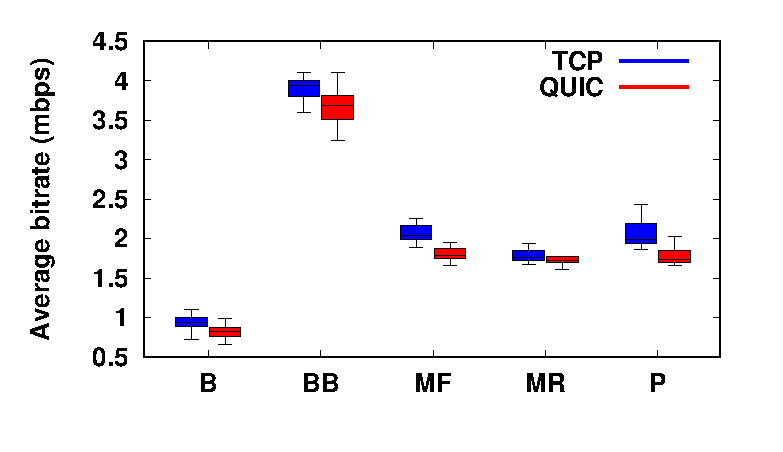
\includegraphics[width=\linewidth]{img/newexp/bitrate_box}
		\caption{\label{fig:chap03s2:averageQuality_n}Average Playback Video Quality for Different ABR Techniques ($p<0.05$ for all the metrics)}
	\end{minipage}\hfill
	\begin{minipage}[t]{0.48\linewidth}
		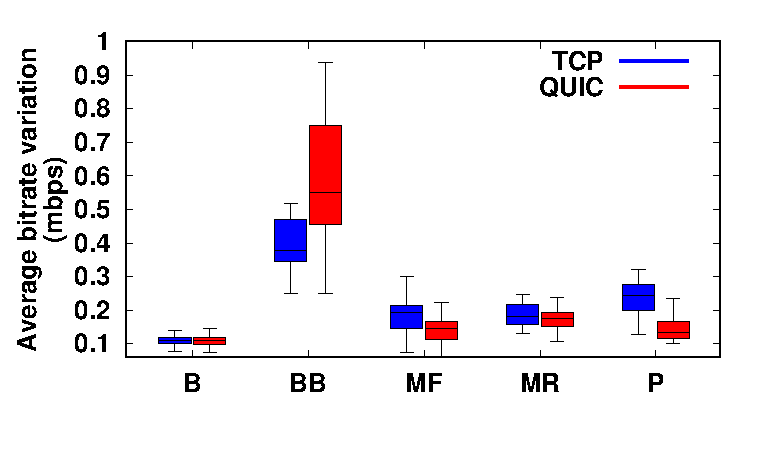
\includegraphics[width=\linewidth]{img/newexp/smooth_box}
		\caption{\label{fig:chap03s2:averageQualityVariation_n}Average Playback Quality Variation for Different \acs{ABR} Techniques ($p<0.05$ for all the metrics except BOLA and MPC-Robust)}
	\end{minipage}

	\begin{minipage}[t]{0.48\linewidth}
		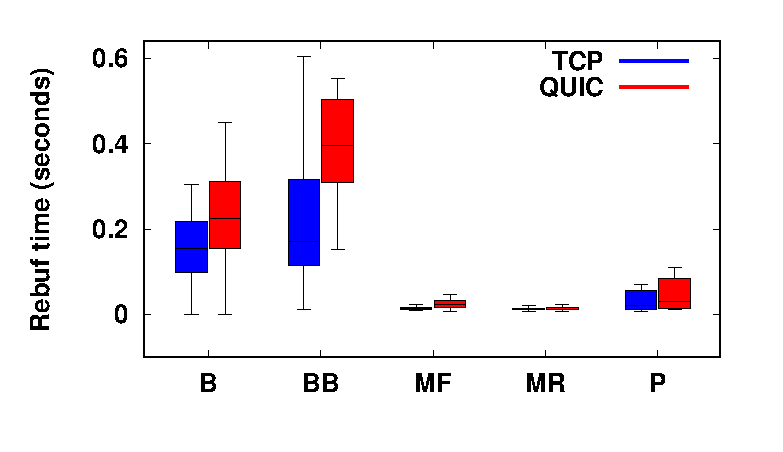
\includegraphics[width=\linewidth]{img/newexp/rebuf_box}
		\caption{\label{fig:chap03s2:RebufferTime_n}Rebuffering Time for Different ABR Techniques ($p<0.05$ for all the metrics except Pensieve and MPC-Robust)}
	\end{minipage}\hfill
	\begin{minipage}[t]{0.48\linewidth}
		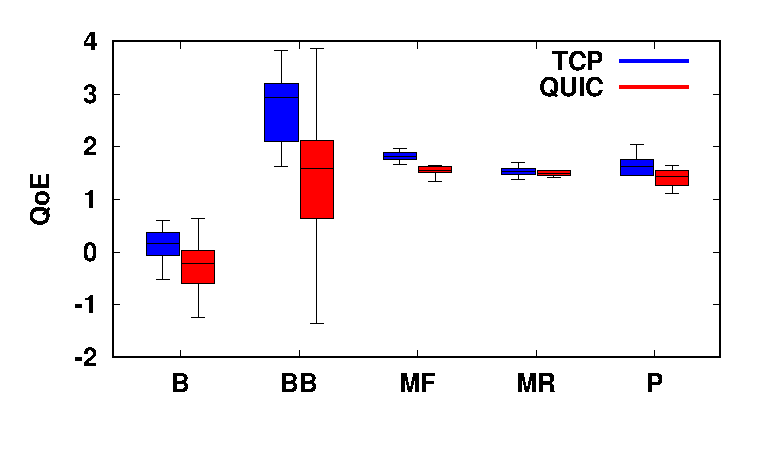
\includegraphics[width=\linewidth]{img/newexp/qoe_box}
		\caption{\label{fig:chap03s2:QOE_n}Overall QoE for Different ABR Techniques ($p<0.05$ for all the metrics except MPC-Robust)}
	\end{minipage}
\end{figure*}

\subsection{Results and Analysis}
We first look into the overall playback video quality and then dig into the details of individual \ac{QoE} metrics. As the data used for this analysis have been collected from realistic experiments, we, therefore, avoid any underlying parametric assumption while checking for the statistical significance of the results. Subsequently, we apply Mann–Whitney U test~\cite{mannwhitney} with non-parametric assumptions on all the metrics and report if the results are statistically significant or not with the hypothesis that DASH/TCP works significantly better than DASH/QUIC\footnote{We use the notation ``DASH/TCP'' to indicate \ac{DASH} over \ac{TCP}; similarly ``DASH/QUIC'' indicates \ac{DASH} over \ac{QUIC}.}. We also run a two-way test to check the alternate hypothesis that DASH/QUIC works significantly better than DASH/TCP.




\subsubsection{Average Video Bitrate}
The distributions of the average playback bitrate for the five \ac{ABR} mechanisms are shown in \fig\ref{fig:chap03s2:averageQuality_n}. For BOLA, we observe that the average video bitrate for DASH/TCP is higher than that of DASH/QUIC. It is known from the existing literature that buffer-based \ac{ABR} mechanisms aggressively use the highest quality levels, which we also observe in \fig\ref{fig:chap03s2:averageQuality_n}. However, we observe that DASH/TCP always performs better than DASH/QUIC. Indeed, the state-of-the-art reinforcement learning based \ac{ABR} mechanism, Pensieve, provides much better quality level on top of \ac{TCP} in comparison to \ac{QUIC}. For all the five \ac{ABR} methods, we observe that the $p$-value is less than $0.05$ for the Mann–Whitney U test, indicating that DASH/TCP performs significantly better than DASH/QUIC in terms of average playback quality.

\subsubsection{Quality Level Fluctuation -- Playback Smoothness}
Next, we observe the average fluctuation in the playback quality levels, which has been shown in \fig\ref{fig:chap03s2:averageQualityVariation_n}. A fluctuation in the quality level indicates less smoothness in the video playback, and, therefore, reduces the \ac{QoE}. We observe that the differences in average quality level fluctuations between DASH/TCP and DASH/QUIC for BOLA and MPC-Robust are statistically insignificant. However, the figure indicates that quality fluctuation with DASH/QUIC is significantly more for buffer-based \ac{ABR}, whereas less for MPC-Fast and Pensieve-based \ac{ABR}, with $p$-value less than $0.05$. This is an interesting observation as we see that the advanced \ac{ABR} techniques, such as MPC-Fast and Pensieve, provide better playback smoothness with DASH/QUIC, although the supported playback quality is lower compared to DASH/TCP.


\subsubsection{Rebuffering Time}
\fig\ref{fig:chap03s2:RebufferTime_n} indicates the rebuffering time for different \ac{ABR} techniques over DASH/TCP and DASH/QUIC. We observe that rebuffering is significantly more with DASH/QUIC for BOLA, buffer-based and MPC-Fast, whereas the differences in rebuffering are statistically insignificant for MPC-Robust and Pensieve. For the buffer-based \ac{ABR} which aggressively download the videos at the highest playback quality, rebuffering is comparatively very high with DASH/QUIC. MPC-Robust and Pensieve show minimal rebuffering, so the differences between DASH/TCP and DASH/QUIC are not statistically significant. We observe that the claim from Google~\cite{langley2017quic} that \ac{QUIC} enables less rebuffering does not hold for all the \ac{ABR} techniques and is very much specific to which \ac{ABR} technique is adopted at the playback client.


\subsubsection{Overall QoE}
Finally, we look into the overall \ac{QoE} computation as shown in \eqn\ref{eqn:chap03s2:QoE}. The overall \ac{QoE} measurements for  all the \ac{ABR} techniques are shown in \fig\ref{fig:chap03s2:QOE_n}. In this experiment, we plot the linear variants of $q(R_n)$ as discussed in the previous section. Our observations from these results are as follows. DASH/TCP provides significantly better \ac{QoE} compared to DASH/QUIC for all the \ac{ABR} algorithms except MPC-Robust where the result is statistically insignificant. This indicates that the recent advanced \ac{ABR} techniques like MPC and Pensieve are more compatible with \ac{TCP} than \ac{QUIC}. Indeed from representations of $q(R_n)$, we can say that the above observations are generic across a wide variation of \ac{QoE} measurements.


